\documentclass[a4paper, 12pt]{article}
\usepackage[spanish]{babel}
\usepackage[utf8]{inputenc}
\usepackage{graphicx}
\usepackage{listings}
\usepackage{xcolor}
\usepackage{float}
\usepackage{array}
\usepackage{multirow}
\usepackage{longtable}
\usepackage[colorlinks=true, linkcolor=black, urlcolor=black, citecolor=black]{hyperref}


\title{Proyecto Final: Sistema de Gestión para Mueblería: Casa Tzalam S.A.}
\author{Integrantes: \\ Flores Herrera Oswaldo \\ Valencia Lerdo Dalia Jimena}
\date{Mayo 2025}

\begin{document}

\begin{titlepage}
    \centering
    
    % Logo UNAM (centrado)
    
\includegraphics[height=3.5cm]{escudo-unam.png}
    \vspace{0.5cm}
    
    % Texto institucional (centrado)
    {\LARGE\textbf{Universidad Nacional Autónoma de}}\\[0.5cm]
    {\LARGE\textbf{México}}\\
    \vspace{0.3cm}
    {\Large\textbf{Facultad de Ingeniería}}
    \vspace{1cm}
    
    % Materia (centrado)
    {\Large Bases de Datos}\\
    \vspace{0.5cm}
    
    % Información del curso (centrado)
    \Large\textbf{Profesor:} Ing. Fernando Arreola Franco\\
    \vspace{0.5cm}
    
    \Large\textbf{Semestre:} 2025-2\\
    \vspace{1cm}
    
    % Título del proyecto (centrado)
    {\Large \textbf{Proyecto Final}}\\
    \vspace{0.3cm}
    {\LARGE \textbf{Sistema de Gestión de Mueblería}}\\
    \vspace{1cm}
    
    % Información del grupo (centrado)
    \Large\textbf{Grupo:} 1\\
    \vspace{0.8cm}
    
    % Alumnos (centrado)
    \Large\textbf{Alumnos:}\\
    Flores Herrera Oswaldo\\
    Valencia Lerdo Dalia Jimena\\
    \vspace{1cm}
    
    % Fecha (alineado izquierda pero dentro de entorno centrado)
    \begin{flushleft}
    \small\textbf{Cd. Universitaria a 25 de Mayo de 2025}
    \end{flushleft}
\end{titlepage}
 


\maketitle

\begin{abstract}
Este documento presenta el diseño e implementación de un sistema de gestión de bases de datos para la mueblería ``Casa Tzalam S.A.'', que busca digitalizar sus operaciones y centralizar la información de sus múltiples sucursales. El sistema permite gestionar artículos, proveedores, ventas, clientes y empleados, cumpliendo con los requerimientos funcionales establecidos. Se implementaron triggers, vistas y un dashboard de visualización para apoyar la toma de decisiones. El proyecto sigue los principios de normalización y garantiza la integridad de los datos mediante restricciones y validaciones.
\end{abstract}
\clearpage 

\tableofcontents

\section{Introducción}
\subsection{Contexto y Problema}
Casa Tzalam S.A. es una reconocida cadena de mueblerías con presencia en 10 estados de la república mexicana. A lo largo de los años, ha crecido gracias a su enfoque en la calidad y el diseño de muebles, pero actualmente enfrenta un reto importante: todos sus registros se llevan de forma física y cada sucursal gestiona su información por separado.
\vspace{5mm}
Esto ha provocado varios problemas, como pérdida de datos, inconsistencias en los inventarios y dificultades para obtener reportes claros y unificados sobre lo que ocurre en toda la empresa.
\vspace{5mm}
Por eso, el proyecto se enfoca en diseñar una base de datos que le permita a Casa Tzalam dar el paso hacia la digitalización. La idea es contar con un sistema centralizado que unifique la información de todas las sucursales y haga más eficiente la operación del negocio.

Con esta propuesta de solución se busca:
\vspace{5mm}
\begin{itemize}
    \item Gestionar el inventario en todas las sucursales
    \item Registrar ventas de manera electrónica
    \item Generar reportes financieros, de forma automática y confiable
    \item Mantener información centralizada de clientes y empleados para un mejor manejo
\end{itemize}

\subsection{Objetivos}
\subsubsection{Objetivo General}
Diseñar e implementar un sistema de gestión de bases de datos que centralice las operaciones de ``Casa Tzalam S.A.'' y que permita manejar eficientemente el registro, consulta, actualización y reporte de la información relacionada con inventarios, ventas, compras, clientes y proveedores, asegurando la integridad, disponibilidad y seguridad de los datos para apoyar la toma de decisiones operativas.

\subsubsection{Objetivos Específicos}
\begin{itemize}
    \item Modelar la estructura de datos que represente todas las entidades del negocio
    \item Implementar mecanismos para garantizar la integridad de la información
    \item Desarrollar procedimientos automatizados para las operaciones recurrentes
    \item Crear un dashboard para visualización de indicadores clave
\end{itemize}

\subsection{Alcance}
El sistema cubrirá:
\begin{itemize}
    \item Gestión de artículos y categorías
    \item Registro de proveedores
    \item Proceso completo de ventas
    \item Administración de clientes
    \item Control de empleados y sucursales
    \item Generación de reportes básicos
\end{itemize}

\section{Plan de Trabajo}
\subsection{Metodología}
Se utilizó una metodología ágil adaptada para proyectos de bases de datos, con las siguientes fases:
\begin{enumerate}
    \item Análisis de requerimientos
    \item Diseño conceptual (MER)
    \item Diseño lógico (MR)
    \item Implementación física
    \item Pruebas y ajustes
    \item Documentación y presentación
\end{enumerate}

\subsection{Cronograma}
\begin{table}[H]
\centering
\begin{tabular}{|l|l|l|l|}
\hline
\textbf{Fase} & \textbf{Responsable} & \textbf{Fecha Inicio} & \textbf{Fecha Fin} \\ \hline
Análisis & Todos & 14-Abr & 20-Abr \\ \hline
Diseño MER & Todos & 21-Abr & 27-Abr \\ \hline
Diseño MR & Todos & 28-Abr & 04-May \\ \hline
Implementación & Todos & 05-May & 17-May \\ \hline
Pruebas & Todos & 18-May & 21-May \\ \hline
Documentación & Todos & 22-May & 24-May \\ \hline
\end{tabular}
\caption{Cronograma del proyecto}
\end{table}

\subsection{Distribución de Trabajo}
    Como un equipo conformado por dos integrantes, adoptamos un enfoque colaborativo en el que ambos participamos activamente en todas las fases del proyecto.
    Desde el análisis de requerimientos hasta la implementación final, nos mativukos involucrados de manera equitativa, asegurando que ambos estuvieramos involucrados en la toma de decisiones y comprendieramos cada una de estas.
\vspace{5mm}
    Dividimos las responsabilidades principales de forma estratégica: uno de nosotros se centró más en el diseño e implementación de la base de datos, mientras que el otro puso mayor atención en el análisis de datos y la creación del dashboard. Aun así, ambos nos involucramos en cada parte del proyecto. Revisamos el trabajo del otro, hicimos sugerencias y colaboramos en tareas como la creación de tablas, el desarrollo de vistas y la programación de triggers.
\vspace{5mm}
    Trabajar en un equipo pequeño fue una ventaja, pudimos comunicarnos constantemente, adaptarnos rápido a los cambios y mantener una buena coordinación. Al estra involucrados en todas las etapas del proyecto, no solo ayudó a lograr un buen resultado, también nos permitió aprender más durante el proceso.
\newpage
\section{Diseño de la Base de Datos}
\subsection{Modelo Entidad-Relación}
El modelo entidad-relación captura las principales entidades del negocio y sus relaciones.

\begin{figure}[h]
    \centering
    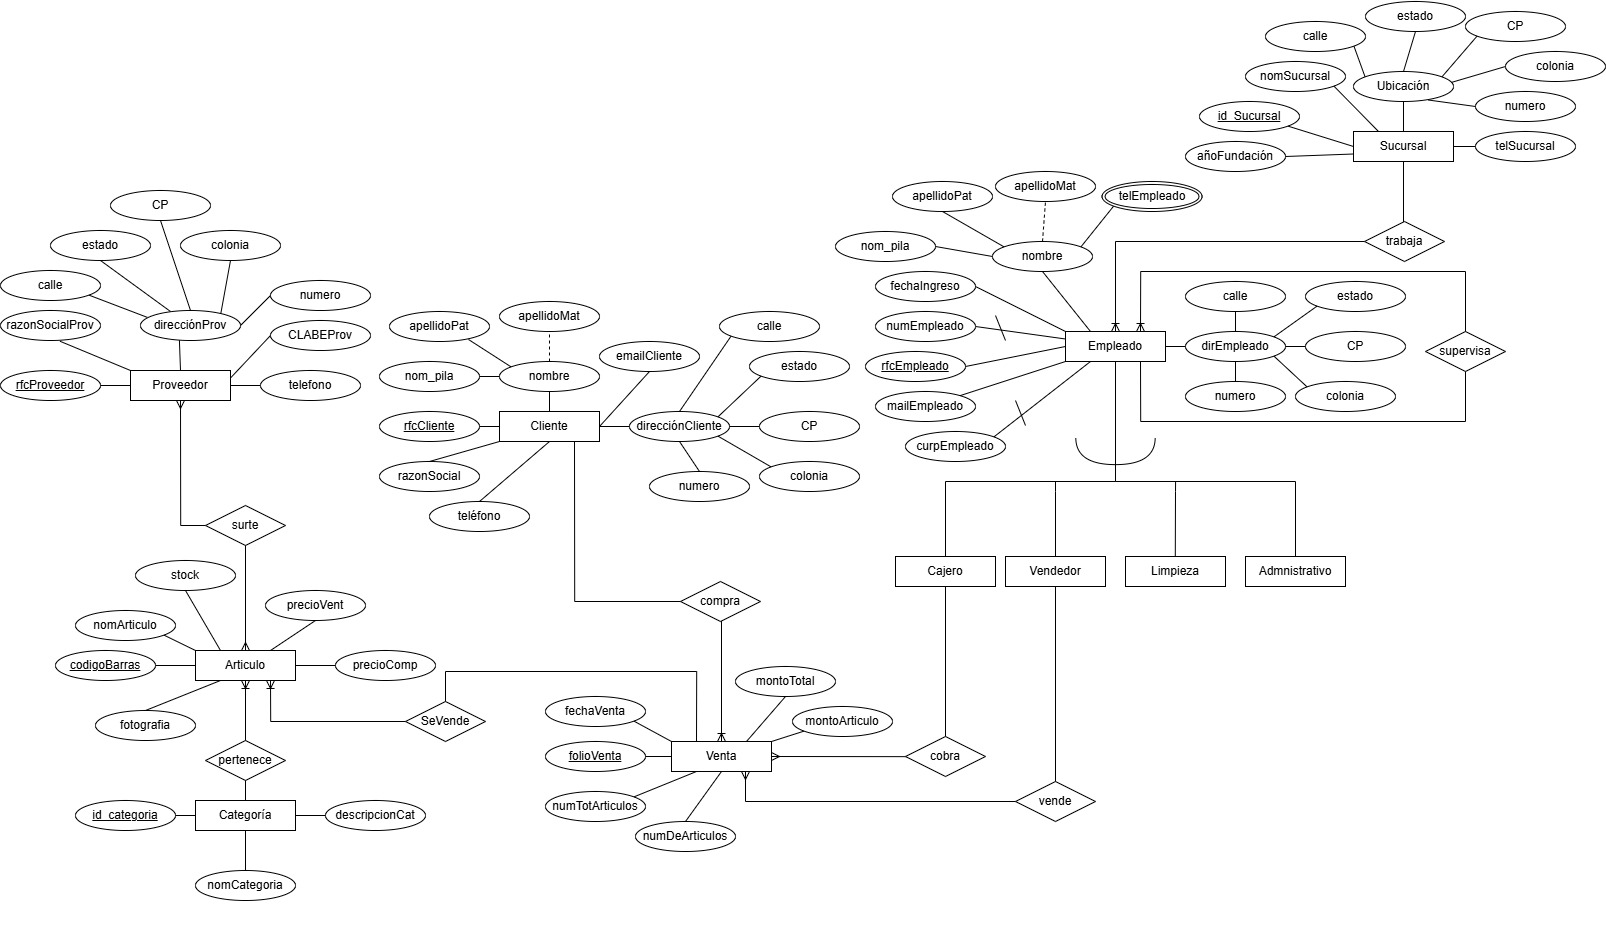
\includegraphics[width=0.9\textwidth]{MER.jpg}
    \caption{Modelo Entidad-Relación del sistema.}
    \label{fig:mer}
\end{figure}

\vspace{5mm}
Principales entidades:



\begin{itemize}
    \item \textbf{Artículo}: Productos que comercializa la mueblería
    \item \textbf{Categoría}: Clasificación de artículos
    \item \textbf{Proveedor}: Empresas que surten los artículos
    \item \textbf{Cliente}: Personas o empresas que compran en la mueblería
    \item \textbf{Empleado}: Personal de la empresa 
    \item \textbf{Sucursal}: Tiendas físicas
    \item \textbf{Venta}: Transacciones comerciales
\end{itemize}

\subsection{Modelo Relacional}
El modelo relacional resultante consta de 8 tablas principales:

\begin{figure}[H]
\centering
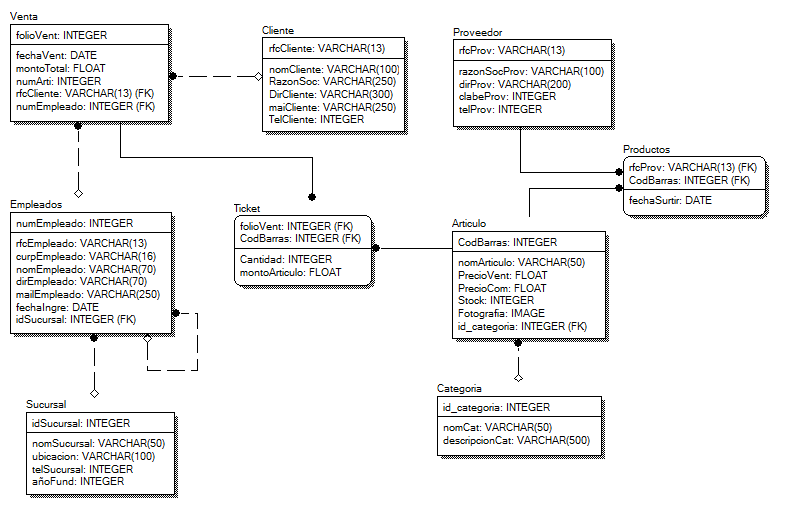
\includegraphics[width=0.9\textwidth]{MR.png}
\caption{Modelo Entidad-Relación del sistema}
\label{fig:mer}
\end{figure}

\subsection{Diccionario de Datos}
A continuación se presenta un fragmento del diccionario de datos completo:

\begin{longtable}{|p{2.5cm}|p{2.5cm}|p{2.5cm}|p{6cm}|}
\hline
\textbf{Tabla} & \textbf{Atributo} & \textbf{Tipo} & \textbf{Descripción} \\ \hline
\endhead

articulo & codigo\_barras & bigint & Identificador único del artículo\\ \hline
articulo & nom\_articulo & varchar(100) & Nombre comercial del artículo \\ \hline
articulo & precio\_venta & numeric(10,2) & Precio al público con 2 decimales \\ \hline
articulo & stock & integer & Cantidad disponible en inventario \\ \hline

categoria & id\_categoria & serial & Llave primaria autoincremental \\ \hline
categoria & nom\_categoria & varchar(100) & Nombre de la categoría \\ \hline

venta & folio\_venta & varchar(10) & Folio con formato MBL-001 \\ \hline
venta & fecha\_venta & timestamp & Fecha y hora de la venta \\ \hline
venta & monto\_total & numeric(10,2) & Suma total de la venta \\ \hline

\caption{Fragmento del diccionario de datos}
\end{longtable}

\section{Implementación}
\subsection{Script de Creación}

Se implementó el siguiente esquema de base de datos en PostgreSQL:

El sistema de gestión para Casa Tzalam S.A. se implementó mediante un conjunto de scripts SQL diseñados para crear y configurar la base de datos en PostgreSQL. 
Estos scripts se organizaron en módulos lógicos que abarcan desde la creación de la estructura básica hasta la programación de funcionalidades.
\vspace{5mm}
El script inicial establece el entorno de la base de datos, configurando la codificación UTF-8 para soportar caracteres especiales y el esquema de búsqueda predeterminado. 
La base de datos se creó desde cero con el nombre DBMB para garantizar un entorno limpio. Las tablas principales incluyen:

\begin{itemize}
  \item \texttt{Artículo}: Contiene información de productos como código de barras, nombre, precios de venta y compra, stock y categoría.
  \item \texttt{Categoría}: Almacena la clasificación de los artículos con campos para nombre y descripción.
  \item \texttt{Cliente}: Registra datos personales, dirección y contacto de los clientes, incluyendo un campo generado para la razón social.
  \item \texttt{Empleado}: Gestiona información del personal, con validación de tipos de empleado mediante una restricción CHECK.
  \item \texttt{Venta} y \texttt{Ticket}: Administran el proceso de ventas, con triggers para actualizar automáticamente los totales y validar el stock.
\end{itemize}


\subsection{Restricciones e Integridad}
 Se definieron restricciones para garantizar la integridad referencial y garantizar la integridad de los datos, como llaves primarias en todas las tablas y llaves foráneas que vinculan artículos con categorías, ventas con empleados y tickets con artículos:

\begin{itemize}
    \item \textbf{LLaves primarias y foráneas}: Para mantener relaciones válidas
    \item \textbf{CHECK constraints}: Para validar dominios (ej. tipo\_empleado)
    \item \textbf{UNIQUE}: Para campos como RFC y CURP de empleados
    \item \textbf{NOT NULL}: Para campos obligatorios
    \item \textbf{Acciones en cascada}: Gestionan automáticamente la propagación o anulación de cambios en relaciones
\end{itemize}

\subsection{Índices}

La creación de índices en las tablas clave de la base de datos, una estrategia fundamental para optimizar el rendimiento del sistema. 
Estos índices funcionan como atajos que permiten acelerar significativamente las operaciones de búsqueda en las columnas más frecuentemente consultadas. 
En concreto, se crea un índice sobre el nombre de los artículos (\textit{idx\_articulo\_nombre}) para agilizar la búsqueda de productos por su denominación, otro sobre el RFC de los clientes (\textit{idx\_cliente\_rfc}) que facilita la localización rápida de clientes específicos, 
un índice en el número de empleado (\textit{idx\_empleado\_num}) que optimiza el acceso a los registros del personal, y finalmente un índice sobre la fecha de venta (\textit{idx\_venta\_fecha}) que mejora el rendimiento de las consultas que filtran información por períodos temporales. 
Estos índices actúan como estructuras organizadas que permiten al motor de la base de datos encontrar rápidamente los registros sin necesidad de escanear todas las filas de las tablas, reduciendo así el tiempo de respuesta de las consultas y mejorando la eficiencia general del sistema, 
especialmente importante en operaciones frecuentes como búsquedas de productos, consulta de historiales de clientes o generación de reportes por períodos específicos.


\subsection{Triggers y Funciones}

Se implementaron varios triggers para automatizar procesos:


\textit{Funciones}
Las funciones  en este sistema están diseñadas para automatizar procesos clave y generar reportes:
\begin{itemize}
    \item \texttt{reporteInventario()}: Analiza el stock de productos, clasificándolo en estados como \textit{``AGOTADO''} o \textit{``BAJO''}, y sugiere acciones de reposición, combinando datos de inventario con ventas recientes.
    
    \item \texttt{venta()}: Gestiona todo el proceso de una transacción: valida empleados, verifica stock, calcula totales, registra la venta y actualiza el inventario, asegurando integridad en cada paso.
    
    \item \texttt{reporteIngresos()}: Genera reportes financieros mensuales por sucursal, mostrando tendencias y comparativas. 
\end{itemize}
Estas funciones encapsulan lógica compleja para simplificar operaciones recurrentes y garantizar consistencia en los datos.

\textit{Triggers}
Los triggers actúan como guardianes automáticos de la integridad de los datos:
\begin{itemize}
    \item \texttt{tr\_validar\_sucursal\_empleados}: Verifica que vendedor y cajero pertenezcan a la misma sucursal antes de registrar una venta, evitando inconsistencias.
    
    \item \texttt{validar\_stock\_articulo}: Rechaza ventas si no hay suficiente inventario, mostrando mensajes claros al usuario.
    
    \item \texttt{actualizar\_totales\_venta}: Mantiene sincronizados los montos totales en la tabla venta cuando se modifican los tickets asociados, asegurando que los cálculos siempre reflejen los detalles actualizados.
\end{itemize}
Estos triggers operan de forma transparente, ejecutándose antes o después de ciertas acciones (\texttt{INSERT/UPDATE/DELETE}) para aplicar reglas de negocio críticas sin intervención manual.

\subsection{Vistas}

Las vistas del sistema son herramientas prácticas que facilitan el trabajo diario:  
\textit{\texttt{vw\_stock\_art}} funciona como un semáforo de inventario, destacando productos con stock bajo o agotados;  
\textit{\texttt{vw\_ticket\_venta}} actúa como un comprobante digital completo, mostrando artículos vendidos, vendedores, sucursal y datos del cliente en un solo lugar;  
y \textit{\texttt{vw\_organigrama}} dibuja el árbol de personal de la empresa, clarificando quién reporta a quién.  
\vspace{5mm}
Estas vistas ahorran tiempo al evitar consultas repetitivas, garantizan que todos usen la misma información actualizada y simplifican la generación de reportes, haciendo más eficiente el análisis de ventas, el control de inventario y la gestión del personal.
\newpage

\section{Aplicación}
\subsection{Dashboard}
El dashboard del sistema integra información clave a través de las siguientes consultas:

\begin{itemize}
    \item \textbf{Ingresos mensuales por sucursal}: Agrupa las ventas por mes y sucursal, mostrando los ingresos totales para un año específico (2025 en este caso), ordenados por sucursal y mes.

    \item \textbf{Artículos más vendidos por categoría}: Proporciona un ranking de productos mostrando las cantidades vendidas e ingresos generados, agrupados por categoría y ordenados por volumen de ventas.

    \item \textbf{Comparativo mensual de sucursales}: Muestra el desempeño de cada sucursal en el mes en curso, incluyendo el número total de ventas e ingresos generados, ordenados por volumen de ingresos.

    \item \textbf{Indicadores clave (KPIs)}: Calcula métricas esenciales como:
    \begin{itemize}
        \item Número total de ventas
        \item Ingresos totales
        \item Ticket promedio
        \item Clientes activos
        \item Artículos con stock bajo
    \end{itemize}
    para los últimos 30 días.

    \item \textbf{Ventas totales por sucursal}: Proporciona una visión consolidada de los ingresos por cada ubicación.
\end{itemize}

Estas vistas proporcionan los datos fundamentales que alimentan las visualizaciones del panel, garantizando información actualizada para la toma de decisiones.

\subsection{Manual de Usuario Básico}

\subsubsection{Registrar una Venta}
Para registrar una nueva venta en el sistema:
\begin{enumerate}
    \item Ejecutar la función \texttt{venta()} con los siguientes parámetros:
    \begin{itemize}
        \item ID del vendedor (ej: \texttt{'EMP002'})
        \item ID del cajero (ej: \texttt{'EMP001'})
        \item RFC del cliente (ej: \texttt{'LORE930606MDF'})
        \item Array de códigos de barras de artículos (ej: \texttt{ARRAY[140433330034, 140433330006]})
        \item Array de cantidades correspondientes (ej: \texttt{ARRAY[2, 1]})
    \end{itemize}
    
    \textbf{Ejemplo:}
    \begin{verbatim}
    SELECT venta(
        'EMP002', 
        'EMP001', 
        'LORE930606MDF',
        ARRAY[140433330034, 140433330006],
        ARRAY[2, 1]
    );
    \end{verbatim}
    
    \item El sistema procesará automáticamente:
    \begin{itemize}
        \item Validación de stock disponible
        \item Cálculo de totales
        \item Actualización de inventario
        \item Generación del folio de venta
    \end{itemize}
\end{enumerate}

\subsubsection{Consultar Stock}
Para verificar el estado del inventario:
\begin{enumerate}
    \item Consultar la vista \texttt{vw\_stock\_art} que muestra:
    \begin{itemize}
        \item Código de barras y nombre del artículo
        \item Precios de venta y compra
        \item Estado de disponibilidad (Disponible/Baja disponibilidad/No disponible)
        \item Cantidad exacta en inventario
    \end{itemize}
    \newpage
    \textbf{Ejemplo básico:}
    \begin{verbatim}
    SELECT * FROM vw_stock_art;
    \end{verbatim}
    \item Para filtrar resultados:
    \begin{itemize}
        \item Por disponibilidad: \texttt{WHERE disponibilidad LIKE 'Baja disponibilidad\%'}
        \item Por categoría: \texttt{WHERE id\_categoria = X}
        \item Por rango de precios: \texttt{WHERE precio\_venta BETWEEN Y AND Z}
    \end{itemize}
\end{enumerate}

\section{Resultados}
\subsection{Resultados Obtenidos}

Durante el desarrollo de nuestro proyecto logramos implementar un sistema que gestionara una base de datos integral de una mueblería, logrando transformar procesos manuales en soluciones automatizadas. Dentro de nuestros resultados mas significativos destacaremos 
\vspace{5mm}
Una centralización eficiente donde consolidamos toda la información operacional ejemplo de ello los inventarios, ventas, clientes y proovedores en una plataforma unificada, eliminando la redundancia y facilitando el acceso a los datos en tiempo real, de igual forma la automatización en los procesos optimizo las tareas criticas como el control de stock, facturación y seguimiento de pedidos, reduciendo errores humanos y mejorando la productividad del negocio esto trae consigo un análisis estratégico de generación de reportes personalizados como lo son ventas por periodo y la producción mas demandada, de igual manera el implementar seguridad e integridad en los datos permitió validar mecanismos como backups periódicos y perfiles de usuario para garantizar la protección y consistencias de la información.
\vspace{5mm}
La implementación de este sistema de gestión de bases de datos no solo resuelve las necesidades operativas inmediatas de la mueblería, sino que establece un marco robusto  en el crecimiento sostenible gracias a la s bases de datos.
Este caso de estudio nos evidencia como la transición hacia un modelo digitalizado centrado en bases de datos estructura de forma útil y moderniza los negocios tradicionales. De igual forma diferencia estratégicamente el impulso a explorar integraciones de este tipo de herramientas para profundizar en el análisis y automatización de decisiones.

\subsection{Dificultades y Soluciones}
\begin{itemize}
    \item \textbf{Problema}: Validación compleja de vendedor y cajero de misma sucursal
    \item \textbf{Solución}: Implementación de trigger \texttt{validar\_sucursal\_empleados}
    
    \item \textbf{Problema}: Generación automática de folios con formato MBL-001
    \item \textbf{Solución}: Uso de secuencia y función de formato en DEFAULT

\item \textbf{Problema}: Actualización dek inventario después de cada venta
\item \textbf{Solución}: Implementación de trigger \texttt{actualizar\_stock\_venta()} y \texttt{actualizar\_stock\_articulo()} que reduce automáticamente el stock al registrar una venta y verifican disponibilidad

\item \textbf{Problema}: Inconsistencias en los totales de ventas al modificar tickets
\item \textbf{Solución}: Implementación del trigger \texttt{tr\_actualizar\_totales} con la función \texttt{actualizar\_totales\_venta()} que:
    \begin{itemize}
        \item Recalcula automáticamente el monto total sumando todos los subtotales de tickets
        \item Actualiza la cantidad total de artículos vendidos
        \item Se ejecuta después de cada inserción, actualización o eliminación en tickets
        \item Garantiza coherencia entre ventas y sus tickets asociados
    \end{itemize}
\end{itemize}

\subsection{Trabajo Futuro}

El sistema implementado ofrece una base sólida para futuras mejoras, comenzando con la integración a plataformas de e-commerce mediante APIs que conectarán nuestra base de datos con sistemas en línea, permitiendo la sincronización en tiempo real de inventarios, precios y pedidos. Este desarrollo puede complementarse con interfaces gráficas más robustas, ya sea mediante un portal web o una aplicación móvil para vendedores, facilitando el acceso remoto a datos, la generación de cotizaciones y la gestión de entregas. Como proyecto culminante, se plantea la migración completa a la nube, aprovechando sus ventajas de escalabilidad automática, mayor capacidad de almacenamiento, mantenimiento simplificado y reducción de costos en infraestructura física, todo ello respaldado por protocolos de seguridad y disponibilidad garantizada.

\section{Conclusiones}

\subsection{Conclusiones Personales}

\textbf{Flores Herrera Oswaldo}

Este proyecto representó un reto significativo pero también una gran oportunidad de aprendizaje. Una de las dificultades más grandes que enfrenté fue el diseño de los triggers para garantizar la integridad de los datos, especialmente en el proceso de ventas, donde era crucial validar el stock, calcular totales y asegurar que vendedor y cajero pertenecieran a la misma sucursal. Al principio, tuvimos problemas con la sintaxis de PL/pgSQL, pero después de investigar y practicar, logramos implementar funciones robustas como \texttt{venta()} y \texttt{actualizar\_totales\_venta()}.
\vspace{5mm}
Uno de los puntos más importantes del proyecto fue la creación del dashboard de visualización, donde pude aplicar mis conocimientos de SQL para generar consultas complejas que muestran KPIs clave como ingresos mensuales y artículos más vendidos. Aprendí la importancia de planificar con anticipación, ya que algunos cambios en el modelo relacional requirieron ajustes en múltiples componentes del sistema. Lo más relevante desde mi punto de vista fue comprobar cómo conceptos teóricos  se traducen en soluciones concretas para la resolución de probelmas reales.

\vspace{5mm}

\textbf{Valencia Lerdo Dalia Jimena}

El desarrollo de este sistema me permitió aplicar conceptos teóricos a un caso real. Uno de los retos más grandes fue normalizar la base de datos para evitar redundancias, especialmente en tablas como \texttt{Artículo} y \texttt{Venta}, donde era fácil caer en diseños denormalizados. Una función que como equipo nos costó mucho implementar fue \texttt{venta()}, ya que requería coordinar múltiples operaciones críticas en una sola transacción.
\vspace{5mm}
Un acierto importante fue la implementación de las vistas, especialmente \texttt{vw\_ticket\_venta}, que simplifica la generación de comprobantes de compra-venta. Me di cuenta de lo útil que es documentar cada paso, ya que cuando revisábamos el código en equipo, tener comentarios claros facilitó la colaboración. Aprendí que la comunicación constante es clave en proyectos colaborativos, y que probar exhaustivamente cada componente evita errores futuros. Este proyecto me demostró el impacto que un buen diseño de bases de datos puede tener en la eficiencia de un negocio.

\appendix
\section{Código Completo}
\subsection{Scripts SQL}

Los scripts completos están disponibles en el repositorio del proyecto:

\begin{itemize}
    \item \texttt{Muebleria.sql}: Backup de la creación de esquema y tablas
    \item \texttt{Carpeta CSV}: Datos de prueba 
    \item \texttt{programacion.sql}: Triggers, funciones y vistas
    \item \texttt{Contenido visual}: Diagramas, imágenes y gráficas
\end{itemize}

\end{document}